\begin{titlingpage}
{
%\definecolor{kugray}{RGB}{102,102,102}
%\definecolor{natgreen}{RGB}{50,93,61}
\thispagestyle{empty}
\newlength{\topma}\setlength{\topma}{-1in}\addtolength{\topma}{-\headsep}\addtolength{\topma}{-\voffset}\addtolength{\topma}{11mm}
\newlength{\sidema}\setlength{\sidema}{-1in}\addtolength{\sidema}{-\hoffset}\addtolength{\sidema}{-\oddsidemargin}\addtolength{\sidema}{-\marginparsep}\addtolength{\sidema}{15mm}
\newlength{\textwa}\setlength{\textwa}{\paperwidth}\addtolength{\textwa}{-35mm}\addtolength{\textwa}{-\textwidth}
\newlength{\textha}\setlength{\textha}{-\textheight}\addtolength{\textha}{\paperheight}\addtolength{\textha}{-11mm}\addtolength{\textha}{-.1\paperheight}
\changepage{\textha}{\textwa}{}{\sidema}{}{-\topmargin}{-\headheight}{\topma}{}
%\setlength{\parindent}{0pt}
\noindent\begin{minipage}[t]{.8\textwidth}
\noindent\raggedright \textcolor{kugray}{\fontspec[Path=fonts/garamond/]{GaramondPremrPro.otf}\addfontfeature{LetterSpace=13.0}\fontsize{18}{17}\selectfont\textsc{university of copenhagen}}

\vspace{.2em}\textcolor{kugray}{\fontspec[Path=fonts/garamond/]{GaramondPremrPro.otf}\addfontfeature{LetterSpace=13.0}\fontsize{15}{17}\selectfont\textsc{niels bohr institute}}
\end{minipage}\hfill\begin{minipage}[t]{32mm}\raggedleft \vspace{16mm} 
\includegraphics[height=44mm]{figures/bionat.pdf}
\end{minipage}


\newlength{\markbump}\setlength{\markbump}{.3\paperwidth}\addtolength{\markbump}{-6mm}
\newlength{\markdown}\setlength{\markdown}{-75mm}\addtolength{\markdown}{0em}\addtolength{\markdown}{\paperheight}\addtolength{\markdown}{.15\paperwidth}
\noindent\makebox[0pt][l]{\hspace{\markbump}\raisebox{-\markdown}[0pt][0pt]{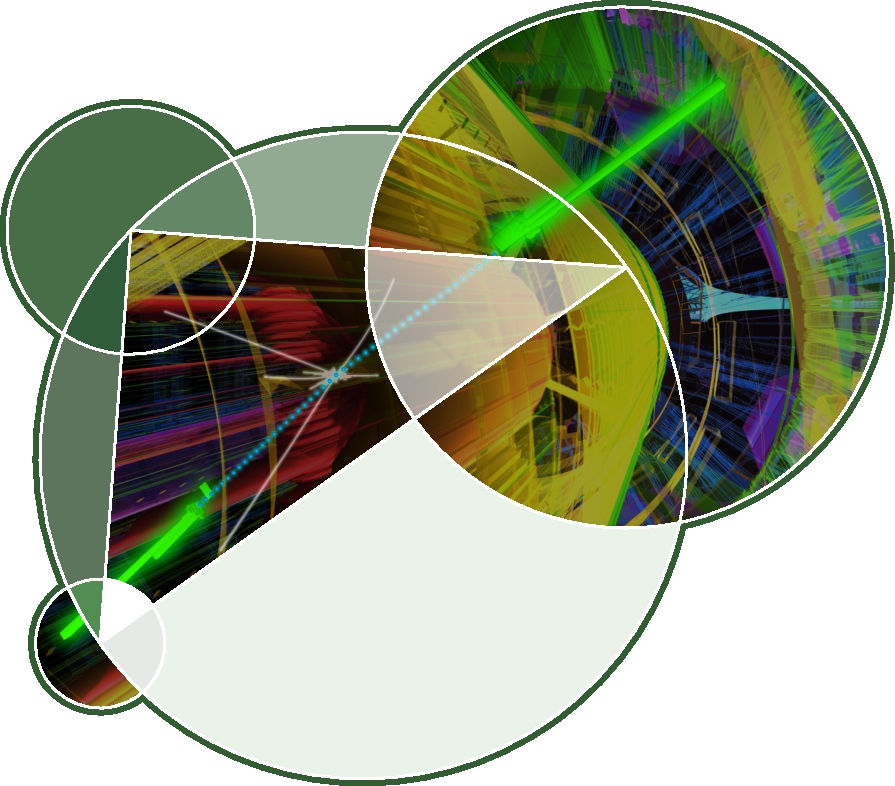
\includegraphics[height=.85\paperwidth]{figures/atlaskugrid2.pdf}}}\makebox[0pt][r]{\raisebox{3.2mm}[0pt][0pt]{\textcolor{natgreen}{\rule{.06\paperwidth}{.7pt}}}}\makebox[0pt][l]{\raisebox{3.2mm}[0pt][0pt]{\textcolor{natgreen}{\rule{.95\paperwidth}{.7pt}}}}





\bigskip

{\sffamily
\begin{hangparas}{0em}{0}
{\textbf{ }

\vspace{2em}}

{\LARGE \textbf{Master's thesis}

\vspace{.3em}}

{\Large Kristoffer Levin Hansen}

\vspace{3em}

{\Huge \raggedright
Search for new physics in diphoton production with the ATLAS detector at the LHC
}
\vfill{}

{\Large Academic advisor: Jørgen Beck Hansen}
\vspace{28em}

\today
\end{hangparas}
}
\clearpage}
\thispagestyle{empty}
  \phantom{p}
\vspace{1.16\textwidth}

\begin{center}

\includegraphics[width=.1\textwidth]{star1}

\vspace{2em}
\begin{minipage}{.6\textwidth}
\emph{``Art is never finished, merely abandoned.''}

\raggedleft\small\sffamily\bfseries\vspace{1em} -- Leonardo da Vinci
\end{minipage}
\end{center}
\clearpage
\end{titlingpage}
\frontmatter

\tableofcontents
\mainmatter

\chapter{Introduction}

Since the late 1960s, our---at times evolving---understanding of the properties and interactions of the fundamental particles has been summarised by the Standard Model of Particle Physics. The Standard Model is formulated in the language of Quantum Field Theory\footnote{Capitalised in anticipation of the imminent use of its common abbreviation, QFT.}, and attempts to combine a theoretical model of quantum mechanical phenomena with an experimental understanding of the properties of fundamental particles and the couplings between them.

An overview of a selection of these properties and interactions is given in fig.~\ref{SMsum}.

\begin{figure}[htp]
\begin{minipage}[b]{.745\textwidth}
\begin{infilsf}
\begin{sffamily}\begin{scriptsize}
\pgfdeclarelayer{back}
\pgfsetlayers{back,main}
\begin{tikzpicture}[yscale=1.8,xscale=0.35]

\tikzstyle{quark}=[font=\footnotesize,white,circle,draw=white,fill=natgreen,inner sep=0pt,minimum size=12pt]
\tikzstyle{gauge}=[font=\footnotesize,white,circle,draw=white,fill=natcomp,inner sep=0pt,minimum size=12pt]
\tikzstyle{higgs}=[font=\footnotesize,white,circle,draw=white,fill=natyellow,inner sep=0pt,minimum size=12pt]
\tikzstyle{lepton}=[font=\footnotesize,white,circle,draw=white,fill=natblue,inner sep=0pt,minimum size=12pt]
\tikzstyle{quarko}=[fill=white,circle,draw=natgreen,inner sep=0pt,minimum size=16pt]
\tikzstyle{gaugeo}=[fill=white,circle,draw=natcomp,inner sep=0pt,minimum size=16pt]
\tikzstyle{higgso}=[fill=white,circle,draw=natyellow,inner sep=0pt,minimum size=16pt]
\tikzstyle{leptono}=[fill=white,circle,draw=natblue,inner sep=0pt,minimum size=16pt]
\tikzstyle{inter}=[kugray!50, ultra thick,cap=rect]
\tikzstyle{under}=[line width=3pt,white]

\draw (-3.5,1.8) -- (-3.5,-1.5) -- (-1.7,-1.5) [snake=zigzag] -- (-.3,-1.5) [snake=none] --  (21,-1.5) -- (21,1.8) -- cycle;
\draw (-3.5,0) node[left] {0} -- +(8pt,0);
\draw (-3.5,1) node[left] {1} -- +(8pt,0);
\draw (-3.5,-1) node[left] {-1} -- +(8pt,0);
\draw (-2,-1.5) -- +(0,2.5pt) +(0,-.9em) node[above] {0};
\foreach \x in {0,1}
\draw (\x*2.303,-1.5) -- +(0,2.5pt) 
    +(0.693,0) -- +(0.693,1.5pt) +(1.1,0) -- +(1.1,1.5pt) 
    +(1.39,0) -- +(1.39,1.5pt) +(1.61,0) -- +(1.61,1.5pt) +(1.79,0) -- +(1.79,1.5pt)
    +(1.95,0) -- +(1.95,1.5pt) +(2.08,0) -- +(2.08,1.5pt) +(2.2,0) -- +(2.2,1.5pt);
\foreach \x in {2,3,...,8}
\draw (\x*2.303,-1.5) -- +(0,2.5pt) +(0,-.9em) node[above] {$10^{\x}$}
    +(0.693,0) -- +(0.693,1.5pt) +(1.1,0) -- +(1.1,1.5pt) 
    +(1.39,0) -- +(1.39,1.5pt) +(1.61,0) -- +(1.61,1.5pt) +(1.79,0) -- +(1.79,1.5pt)
    +(1.95,0) -- +(1.95,1.5pt) +(2.08,0) -- +(2.08,1.5pt) +(2.2,0) -- +(2.2,1.5pt);
\draw (0,-1.5) -- +(0,2.5pt) +(0,-.9em) node[above] {1};
\draw (2.303,-1.5) -- +(0,2.5pt) +(0,-.9em) node[above] {10};
\draw (9*2.303,-1.5) -- +(0,2.5pt) +(0,-.9em) node[above] {$10^9$};
\node at (-4.8,1.7) [rotate=90,left] {Electromagnetic charge [e]};
\node at (21,-1.8) [left] {Mass [eV/c$^2$]};
\draw (7.74,0.667) node [quarko] (u) {} node {\tikz {\fill[natgreen] (0,0) -- ++(0,8pt) arc (90:-90:8pt) -- cycle; \draw +(180:8pt);}} node [quark] {u};
\draw (8.48,-0.333) node [quarko] (d) {} node {\tikz {\fill[natgreen] (0,0) -- ++(0,8pt) arc (90:-90:8pt) -- cycle; \draw +(180:8pt);}} node [quark] {d};
\draw (14.06,0.667) node [quarko] (s) {} node {\tikz {\fill[natgreen] (0,0) -- ++(0,8pt) arc (90:-90:8pt) -- cycle; \draw +(180:8pt);}} node [quark] {s};
\draw (11.46,-0.333) node [quarko] (c) {} node {\tikz {\fill[natgreen] (0,0) -- ++(0,8pt) arc (90:-90:8pt) -- cycle; \draw +(180:8pt);}} node [quark] {c};
\draw (18.97,0.667) node [quarko] (t) {} node {\tikz {\fill[natgreen] (0,0) -- ++(0,8pt) arc (90:-90:8pt) -- cycle; \draw +(180:8pt);}} node [quark] {t};
\draw (15.25,-0.333) node [quarko] (b) {} node {\tikz {\fill[natgreen] (0,0) -- ++(0,8pt) arc (90:-90:8pt) -- cycle; \draw +(180:8pt);}} node [quark] {b};
\draw (-2,0) ++(100:6.5pt) ++(-4.47pt,0) node (gamma) [gaugeo] {} node {\tikz {\shade[top color=white,bottom color=natcomp] (0,0)  +(-80:12pt) -- +(-45:8pt) arc (-45:-115:8pt) -- cycle; \filldraw[natcomp] (0,0) circle (8pt); \draw +(100:12pt);}} node [gauge] {$\gamma$};
\draw (-2,0) ++(-80:6.5pt) ++(4.47pt,0) node [gaugeo] (g) {} node {\tikz {\shade[top color=natcomp,bottom color=white] +(100:12pt) -- +(135:8pt) arc (135:65:8pt) -- cycle; \filldraw[natcomp] (0,0) circle (8pt); \draw +(-80:12pt);}} node [gauge] {g};
\draw (-2,0) node {\tikz \fill[natcomp] circle (1pt);};
\draw (18.33,0) ++(100:6.5pt) ++(-4.47pt,0) node [gaugeo] (Z) {} node {\tikz {\shade[top color=white,bottom color=natcomp] (0,0)  +(-80:12pt) -- +(-45:8pt) arc (-45:-115:8pt) -- cycle; \filldraw[natcomp] (0,0) circle (8pt); \draw +(100:12pt);}} node [gauge] {Z};
\draw (18.20,1) node [gaugeo] (W+) {} node {\tikz {\filldraw[natcomp] (0,0) circle (8pt);}} node [gauge] {\tiny W$^+$};
\draw (18.20,-1) node [gaugeo] (W-) {} node {\tikz {\filldraw[natcomp] (0,0) circle (8pt);}} node [gauge] {\tiny W$^-$};
\draw (18.65,0)  ++(-80:6.5pt) ++(4.47pt,0) node [higgso] (H) {} node {\tikz {\shade[top color=natyellow,bottom color=white] +(100:12pt) -- +(135:8pt) arc (135:65:8pt) -- cycle; \draw +(-80:12pt); \draw[natyellow] (0,0) circle (8pt);}} node [higgs] {H};
\draw (18.33,0) node {\tikz \fill[natcomp] circle (1pt);};
\draw (18.65,0) node {\tikz \fill[natyellow] circle (1pt);};
\draw (0.79,0) node [leptono] (ve) {} node {\tikz {\fill[natblue] (0,0) -- ++(0,8pt) arc (90:-90:8pt) -- cycle; \draw +(180:8pt);}} node [lepton] {$\nu_{\text e}$};
\draw (5.14,0) node [leptono] (vmu) {} node {\tikz {\fill[natblue] (0,0) -- ++(0,8pt) arc (90:-90:8pt) -- cycle; \draw +(180:8pt);}} node [lepton] {$\nu_\mu$};
\draw (9.65,0) node [leptono] (vtau) {} node {\tikz {\fill[natblue] (0,0) -- ++(0,8pt) arc (90:-90:8pt) -- cycle; \draw +(180:8pt);}} node [lepton] {$\nu_\tau$};
\draw (6.24,-1) node [leptono] (e) {} node {\tikz {\fill[natblue] (0,0) -- ++(0,8pt) arc (90:-90:8pt) -- cycle; \draw +(180:8pt);}} node [lepton] {e};
\draw (11.57,-1) node [leptono] (mu) {} node {\tikz {\fill[natblue] (0,0) -- ++(0,8pt) arc (90:-90:8pt) -- cycle; \draw +(180:8pt);}} node [lepton] {$\mu$};
\draw (14.39,-1) node [leptono] (tau) {} node {\tikz {\fill[natblue] (0,0) -- ++(0,8pt) arc (90:-90:8pt) -- cycle; \draw +(180:8pt);}} node [lepton] {$\tau$};

\begin{pgfonlayer}{back}
\node at (12,1) [inner sep=0] (uqs) {};
\node at (20.7,.6) [inner sep=0] (qgnode) {};
\draw [inter] (u) to[out=0,in=270,max distance=7pt]  (uqs);
\draw [inter] (s) to[out=170,in=270,max distance=4pt] (uqs);
\draw [inter] (t) to[out=190,in=270,max distance=25pt] (uqs);
\draw [inter] (d) to[out=5,in=270,max distance=30pt] (uqs);
\draw [inter] (c) to[out=60,in=270,max distance=10pt] (uqs);
\draw [inter] (b) to[out=170,in=270,max distance=20pt] (uqs)
                  to[out=90,in=40,max distance=17pt] (g);
\draw (g) node[below right] {\tikz {\draw [inter] (0,0) to[in=-40,out=-90,min distance=20pt] (0,0);}};
\draw [inter] (uqs) to[out=90,in=30,max distance=15pt] (gamma);
\draw [inter] (uqs) to[out=90,in=150,max distance=7pt] (W+);
\draw [inter] (uqs) .. controls (12,1.4) and (20.7,1.7) .. (qgnode.south)
                    to[out=270,in=10,max distance=7pt] (Z);
\draw [inter] (qgnode) to[out=270,in=20,max distance=10pt] (H);
\draw [inter] (qgnode) to[out=270,in=20,max distance=30pt] (W-);

\draw [under] (gamma) -- ++(15,0) node [inner sep=0] (gamw) {};
\draw [under] (gamw.west) to[out=0,in=90,max distance=30pt] (W-);
\draw [under] (gamw.west) to[out=0,in=250,max distance=20pt] (W+);
\draw [inter] (gamma) -- (gamw.east);
\draw [inter] (gamw.west) to[out=0,in=250,max distance=20pt] (W+);
\draw [inter] (gamw.west) to[out=0,in=90,max distance=30pt] (W-);

\node at (17,-.3) [inner sep=0] (wz-) {};
\node at (17,.6) [inner sep=0] (wz+) {};
\draw [under] (wz-) -- (wz+) to[out=270,in=160,max distance=10pt] (Z);
\draw [under] (H) to[out=30,in=-5,min distance=30pt] (W+);
\draw [inter] (W-) to[out=160,in=270,max distance=10pt] (wz-)
           to (wz+.north) to[out=90,in=200,max distance=10pt] (W+);
\node [above right] at (W+) {\tikz {
    \draw[under] (0,0) to[out=40,in=90,min distance=20pt] (0,0);
    \draw[inter] (0,0) to[out=40,in=90,min distance=20pt] (0,0);}};
\draw [inter] (wz-) to[out=90,in=200,max distance=10pt] (Z);
\draw [inter] (wz+) to[out=270,in=160,max distance=10pt] (Z);
\draw [inter] (W-) -- (H);
\draw (W-) node[below right] {\tikz {\draw [inter] (0,0) to[in=-40,out=-90,min distance=20pt] (0,0);}};
\draw [inter] (H) to[out=50,in=-10,max distance=5pt] (Z);
\draw [inter] (H) to[out=30,in=-5,min distance=30pt] (W+);

\draw (tau) ++(1.5,.25) node [inner sep=0] (lepga) {};
\draw [inter] (tau) to[out=70,in=180,max distance=3pt] (lepga)
                    to[out=0,in=270,max distance=10pt] (wz-);
\draw [inter] (mu) to[out=70,in=180,max distance=3pt] ++(1.5,.25) -- (lepga);
\draw [inter] (e) to[out=70,in=180,max distance=3pt] ++(1.5,.25)
              node [inner sep=0] (ega) {} -- (lepga);
\draw [inter] (lepga) to[out=0,in=152,max distance=10pt] (W-);

\draw (vmu) ++(-1.5,-.25) node [inner sep=0] (neul) {};
\draw [inter] (vmu) to[out=250,in=0,max distance=3pt] (neul);
\draw [inter] (vtau) to[out=185,in=0,min distance = 30pt] (neul);
\draw [inter] (ve) -- ++(0,-.5) node [inner sep=0] (neud) {};
\draw [inter] (neul.east) to[out=180,in=90,max distance=7pt] (neud);
\draw [inter] (neud.north) to [out=270,in=180,max distance=10pt] (ega);

\draw (g) ++(-1,0) node [inner sep=0] (gamlep) {};
\draw [inter] (e) to [out=250,in=0,max distance=3pt] ++(-1.5,-.25)
              node (lepneu) [inner sep=0] {};
\draw [inter] (mu) to[out=250,in=0,max distance=3pt] ++(-1.5,-.25) -- (lepneu);
\draw [inter] (tau) to[out=250,in=0,max distance=3pt] ++(-1.5,-.25) -- (lepneu);
\draw [inter] (lepneu.east) to[out=180,in=270,max distance=20pt] (neud.north);
\draw [inter] (lepneu) to[out=180,in=270,max distance=30pt] (gamlep);
\draw [inter] (gamma) to[out=230,in=90] (gamlep.south);
\end{pgfonlayer}

\draw[inter,cap=round] (-2,1) -- (0,1) node[right,kugray] {Interactions};

\draw (-1,1.4) node [quarko] (n) {} node {\tikz {\fill[natgreen] (0,0) -- ++(0,8pt) arc (90:-90:8pt) -- cycle; \draw +(180:8pt);}} node [quark] {n};
\node at (n) {\tikz {\draw [white,postaction={decorate,decoration={text along path,text align=center,text={|\tiny|Spin}}}] ++(270:10pt) arc (270:90:10pt); \draw (-1,0) (1,0);}};
\begin{scope}
\clip (n.center) -- ++(2,0) -- ++(0,.2) -- ++(-2,0) -- cycle;
\draw (n) node [gaugeo] {} node {\tikz {\filldraw[natcomp] (0,0) circle (8pt);}} node [gauge] {n};
\end{scope}
\begin{scope}
\clip (n.center) -- ++(2,0) -- ++(0,-.2) -- ++(-2,0) -- cycle;
\draw (n) node [leptono] {} node {\tikz {\fill[natblue] (0,0) -- ++(0,8pt) arc (90:-90:8pt) -- cycle; \draw +(180:8pt);}} node [lepton] {n};
\end{scope}
\begin{scope}
\clip (n.center) -- ++(-2,0) -- ++(0,-.2) -- ++(2,0) -- cycle;
\draw (n) node [higgso] {} node {\tikz {\shade[top color=natyellow,bottom color=white] +(100:12pt) -- +(135:8pt) arc (135:65:8pt) -- cycle; \draw +(-80:12pt); \draw[natyellow] (0,0) circle (8pt);}} node [higgs] {n};
\end{scope}

\draw (n) ++(160:20pt) node [right,natgreen] {\tiny Quarks};
\draw (n) ++(-160:20pt) node [right,natyellow] {\tiny Higgs boson};
\draw (n) ++(0:20pt) node [above right,natcomp] {\tiny Gauge bosons};
\draw (n) ++(0:20pt) node [below right,natblue] {\tiny Leptons};

\end{tikzpicture}
\end{scriptsize}\end{sffamily}
\end{infilsf}
\end{minipage}
\hfill\begin{minipage}[b]{.25\textwidth}
\caption{An overview of the particles of the Standard Model. The particles are arranged by mass and charge. Colour indicates particle type, the filling of the border indicates the spin of particles and lines are drawn between those particles that the Standard Model describes interactions between. The currently known maximum bounds on neutrino masses have been used to place the neutrinos in the mass direction. Table values from \cite{wikism}.\label{SMsum}}
\end{minipage}
\end{figure}

In its current form, the Standard Model makes no attempt to explain any physics beyond this.\footnote{The overview in figure~\ref{SMsum} includes massive neutrinos, which have been found experimentally, even though the Standard Model does not at present include them. There are, however, several proposed methods of extending the SM to do so.} The most obvious missing element is gravity, which finds no obvious expression in terms of Quantum Field Theory. Other seemingly missing elements come from astronomy, which bring observational evidence of a number of phenomena, such as dark matter and dark energy, which seem to require an explanation from within the realm of physics that the Standard Model describes, but for which the Standard Model offers no obvious source.

Disregarding these issues, which may be considered external its scope, the Standard Model has been remarkably successful as a model for high energy particle physics, withstanding decades of experimental tests and correctly predicting the existence and properties of several particles.\footnote{Most recently, the existence of the Higgs boson was confirmed experimentally. At the time of writing, confirmation of its predicted properties is still a work in progress.} In spite of those successes, the Standard Model is not without its issues.

As it is formulated, the SM depends on at least 19 numerical constants,\footnote{Not counting any additional constants needed to account for neutrino masses.} the value of which must be determined experimentally, since the model offers no insight into the origin of or relations between them. Worse still, as the SM is a perturbative model, higher order corrections, which tend to increase the predicted Higgs mass with no constraint save the Planck energy, must be included in the theory. To arrive at the observed Higgs mass in spite of this tendency, either some unknown physics exist between the Higgs mass scale and the Planck scale to constrain the Higgs mass, or the bare mass and couplings of the Higgs boson are very finely tuned to cancel the higher order contributions. This is one example of the hierarchy problem.

In the first case, we will obviously want to search for evidence of the postulated new, high-energy physics. In the latter case, we might expect\footnote{Or \emph{hope for}, depending on how invested we happen to be in the question of fine--tuning.} there to be some additional mechanism within the Standard Model that ensures that the bare Higgs mass and the other free parameters of the SM are given the proper value. Again, we will want to search for physics outside what is currently described by the SM, as a clue to what that mechanism might be.

There is also the possibility that neither of those mechanisms exist, since the Standard Model, strictly speaking, does not require them. In that case a search for new physics that discovers nothing is still a valuable, albeit less illuminating, result.

In this thesis, we shall approach the task of searching for physics beyond the Standard Model by introducing to it an extension via the effective Lagrangian approach. Specifically, we will introduce a $q\bar q\rightarrow\gamma\gamma$ point interaction, and then simulate collision experiments with the new interaction at various strengths, to see how the outcome is affected. We can then, finally, compare the results of those pseudoexperiments to the results of actual collision experiments performed at \textsc{cern}'s Large Hadron Collider, and look for signs of the same effects there.